%!TEX root = ../dissertation.tex
\begin{savequote}[75mm]
A good idea is about ten percent and implementation and hard work, and luck is 90 percent.
\qauthor{Guy Kawasaki}
\end{savequote}

\chapter{Implementation}
This chapter is about the implementation with Apache Storm to solve the defined queries and to do the benchmarks.
The idea of the test scenario is to use "OSM Augmented Diffs" as a stream.
This diffs extend the ordinary minutely diffs of OSM with more information.
The result contains all the nodes, ways and relations changed durring the time periode.

\newpage

\section{Test Setup}
For the implementation there is a given test setup.
The Open Street Map Augmented diffs are minutelly collected by a script executed as a cron job.
The script acts as an producer for Kafka and the data is now accessible from these message queue.
Furthermore the data is ready to be consumed by the stream processing engine and in this case ready for Apache Storm.

\begin{figure}[H]
\centering
\captionsetup{justification=centering}
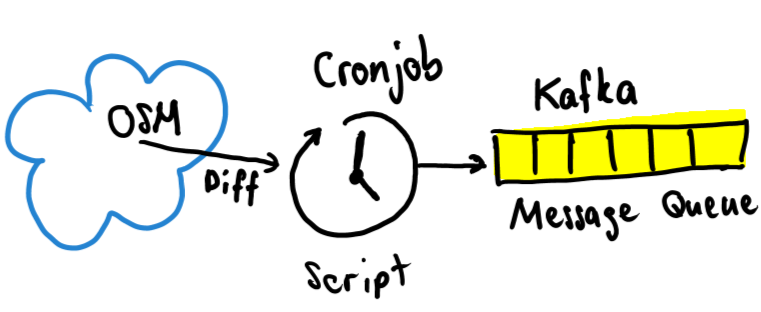
\includegraphics[width=0.6\textwidth]{images/test_setup.png}
\caption[Test setup]{Test setup}
\end{figure}


\section{Queries}
The following list is about the queries which has to be done on the Augmented Diff stream.

\begin{itemize}
\item[A)] Leader board of top 10 OSM active users
\item[B)] Leader board of top 10 OSM objects added
\item[C)] Node objects with suspicious keys and values
\item[D)] Way objects with only user tag "area=yes" without other user tags
\end{itemize}

\subsection{A) Leader board of top 10 OSM active users}
It's about users who created or updated any OSM nodes all around the world.
The users are identified by the tags "uid" and "user".

\subsection{B) Leader board of top 10 OSM objects added}
Count all the created or updated nodes grouped by a combination of key and value.
An example for this is "amenity=bench".

\subsection{C) Node objects with suspicious keys and values}
Detection of vandalism and unwanted bad actions in OpenStreetMap is a very difficult topic.
Thus we focus on "Quality Assurance Monitoring" by filtering for suspicious tags of node or way elements.
As an example for this issues are ";" in Tags like "crossing=island;uncontrolled".

\subsection{D) Way objects with only user tag "area=yes" without other user tags}
The point D) also deals with the vandalism problems.


\newpage
\section{Topic of the queries}


\newpage
\section{Benchmark}
\begin{figure}[H]
\centering
\captionsetup{justification=centering}
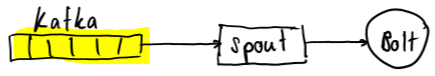
\includegraphics[width=0.4\textwidth]{images/benchmark_topic1.png}
\caption[Benchmark 1 Bolt]{Benchmark 1 Bolt}
\end{figure}


\begin{figure}[H]
\centering
\captionsetup{justification=centering}
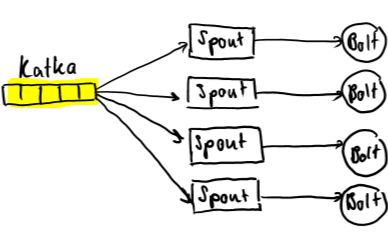
\includegraphics[width=0.4\textwidth]{images/benchmark_topic2.png}
\caption[Benchmark 4 Bolts]{Benchmark 4 Bolts}
\end{figure}


\begin{figure}[H]
\centering
\captionsetup{justification=centering}
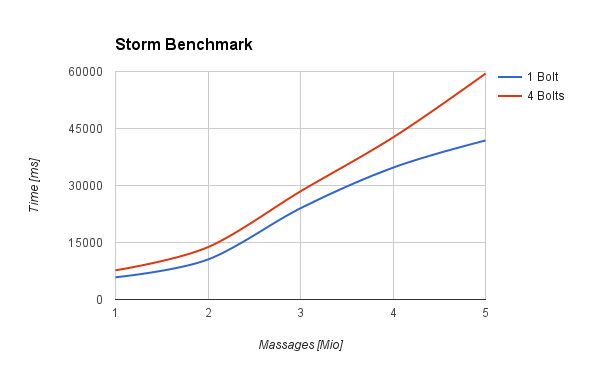
\includegraphics[width=0.9\textwidth]{images/benchmark.png}
\caption[Benchmark Diagramm]{Benchmark Diagramm}
\end{figure}








